\subsection{Поиск рейса}

\textbf{Акторы:} Пользователь, системы авиакомпаний, предоставляющих информацию о полетах

\textbf{Краткое описание:} Пользователь ищет рейс по его параметрам

\textbf{Главная последовательность:} \textbf{Пользователь} вводит известную информацию о рейсе. \textbf{Система авиакомпании} 
предоставляет информацию по данному рейсу. Если рейса с такими пармаметрами нет, то выводится ошибка.

\textbf{Альтернативные последовательности:} \textbf{Пользователь} вручную ищет рейс на онлайн-табло. При нажатии
на него высвечивается информация по нему.

\textbf{Предусловия:} -

\textbf{Постусловия:} -

\textbf{Точки расширения:} -




\subsection{Просмотр пользователем информационных страниц}

\textbf{Акторы:} Пользователь

\textbf{Краткое описание:} Пользователь просматривает информацию, изложенную на информационных страницах

\textbf{Главная последовательность:} \textbf{Пользователь} просматривает тексты на информационных
страницах.

\textbf{Альтернативные последовательности:} Переход на другую информационную страницу с нынешней.

\textbf{Предусловия:} Пользователь находится на одной из информационных страниц

\textbf{Постусловия:} -

\textbf{Точки расширения:} Прецедент 4.9: Навигация между страницами сайта.




\subsection{Заполнение формы}

\textbf{Акторы:} Пользователь, администраторы

\textbf{Краткое описание:} Пользователь запоняет анкету соискателя

\textbf{Главная последовательность:} \textbf{Пользователь} переходит на страницу формы и заполняет её.
\textbf{Пользователь} отправляет форму обратной связи или
анкеты соискателя.\textbf{Администратор} принимает данные из формы.

\textbf{Альтернативные последовательности:} -

\textbf{Предусловия:} Пользователь находится в разделе "Для бизнеса" на странице Соискателя

\textbf{Постусловия:} Форма хранится в базе заявок аэропорта

\textbf{Точки расширения:} -




\subsection{Пользователь бронирует билеты}

\textbf{Акторы:} Пользователь, Платежная система, Модули: Публичный, Биллинг, Почтовый, Билетер

\textbf{Краткое описание:} Пользователь покупает билет

\textbf{Главная последовательность:} 
\begin{enumerate}
      \item \textbf{Клиент} выбирает рейс.
      \item \textbf{Клиент} заполняет форму и отправляет ее
            в \textbf{Публичный}.
      \item \textbf{Публичный} бронирует билет, используюя
            сервис \textbf{Билетер}.
      \item \textbf{Публичный} просит у \textbf{Биллинга}
            форму для ввода реквизитов для оплаты.
      \item \textbf{Биллинг} регистрирует факт запросы формы
            для оплаты и просит \textbf{Платежную систему}
            дать форму, после чего пересылает ее
            \textbf{Публичному}, а тот \textbf{Клиенту}.
      \item \textbf{Клиент} вводит реквизиты карты и нажимает
            отправить, данные отправляются в 
            \textbf{Платежную систему}
      \item \textbf{Клиент} просит предоставить услугу у
            \textbf{Публичного}.
      \item \textbf{Публичный} справшивает у \textbf{Биллинга},
            как там с оплатой дела.
      \item \textbf{Биллинг} справшивает у \textbf{Платежной системы},
            как там с оплатой дела.
      \item Если все ОК, то
            \begin{enumerate}
                  \item \textbf{Биллинг} закрывает транзакцию, которую
                        открыл при регистрации запроса на платеж,
                        если фейл, то фейлит транзакцию, если ХЗ,
                        то отвечает ХЗ.
                  \item Если все ОК \textbf{Публичный} просит
                        \textbf{Билетера} выдать билет.
                  \item \textbf{Билетер} отмечает забронированный
                        билет как купленный и просит \textbf{Почтового},
                        отправить билет на почту \textbf{Пользователя}.
            \end{enumerate}
      \item Если ошибка с оплатой, то
            \begin{enumerate}
                  \item \textbf{Публичный} просит \textbf{Билетера}
                        снять бронь, и отвечает \textbf{Клиенту},
                        что тот проиграл
            \end{enumerate}
      \item Если ХЗ, что там с оплатой, то
            \begin{enumerate}
                  \item \textbf{Публичный} просит \textbf{Билетера}
                        снять бронь, и отвечает \textbf{Клиенту},
                        что тот проиграл
            \end{enumerate}
      \item ХЗ, как-то ждем, что-то делаем асинхронно,
            успокаиваем пользователя
\end{enumerate}

\textbf{Альтернативные последовательности:} Пользователь покупает билет у другой организации предоставляющей
услугу покупки билета.

\textbf{Предусловия:} Пользователь зарегистрирован и находится на странице покупки билетов.

\textbf{Постусловия:} Билет отправляется пользователю и становится недоступным для брони/покупки в других системах(включая разрабатываемую).

\textbf{Точки расширения:} -




\subsection{Бронирование пользователем парковочного места}

\textbf{Акторы:} Пользователь, система бронирования парковочных мест

\textbf{Краткое описание:} Пользователь бронирует праковочное место

\textbf{Главная последовательность:} 
\begin{enumerate}
      \item \textbf{Пользователь} выбирает промежуток времени, на который планирует забронировать парковочное место. 
      \item \textbf{Система бронирования парковочных мест} предоставляет список свободных мест на введенный промежуток времени.
      \item \textbf{Пользователь} выбирает место из доступных.
      \item Место бронируется в \textbf{Системе}.
      \item \textbf{Пользователь} получает номер бронирования.
\end{enumerate}

\textbf{Альтернативные последовательности:} Пользователь на месте бронирует место. \textbf{Администратор} вносит место в \textbf{Систему} в качестве забронированного.

\textbf{Предусловия:} Пользователь зарегистрирован и находится на странице паркинга

\textbf{Постусловия:} Место бронируется и становится недоступно для брони на зарезервированный промежуток времени.

\textbf{Точки расширения:} -




\subsection{Оплата пользователем парковочного места}

\textbf{Акторы:} Пользователь, платежная система

\textbf{Краткое описание:} Пользователь оплачивает парковочное место

\textbf{Главная последовательность:}
\begin{enumerate}
      \item \textbf{Пользователь} вводит номер брони.
      \item Его переводит на страницу оплаты \textbf{Платёжной системы}
      \item \textbf{Пользователь} вводит данные карты для оплаты.
      \item \textbf{Пользователь} оплачивает место.
\end{enumerate}

\textbf{Альтернативные последовательности:} Пользователь на месте оплачивает место. 
\textbf{Администратор} вносит место в \textbf{Систему} в качестве оплаченного.

\textbf{Предусловия:} Если пользователь еще не забронировал место, то сначал выполняется Прецедент-4.5 Бронирование пользователем 
парковочного места. У пользователя имеется номер брони парковочного места.

\textbf{Постусловия:} Место предоставляется пользователю на зарезервированный промежуток времени.

\textbf{Точки расширения:} Прецедент-4.5 Бронирование пользователем парковочного места.




\subsection{Регистрация на сайте}

\textbf{Акторы:} Пользователь

\textbf{Краткое описание:} Пользователь регистрируется на сайте Домодедово

\textbf{Главная последовательность:} \textbf{Пользователь} заполняет персональные данные на странице регистрации.
Если данные корректны, то у него появлется свой кабинет. Иначе выводится сообщение о некорректности данных.

\textbf{Альтернативные последовательности:} -

\textbf{Предусловия:} -

\textbf{Постусловия:} Личный кабинет пользователя регистрируется в системе аэропорта.

\textbf{Точки расширения:} -




\subsection{Вход в личный кабинет}

\textbf{Акторы:} Пользователь

\textbf{Краткое описание:} Пользователь входит в свой личный кабинет.

\textbf{Главная последовательность:} \textbf{Пользователь} заполняет почту и пароль в специальном окне-форме. Если данные корректны, то 
пользователь получает доступ к кабинету, иначе выводится сообщение о некорректности введенных данных и предлагает пользователю регистрацию
(Прецедент-4.7 Регистрация на сайте),восстановление пароля и предложение ввести заново.

\textbf{Альтернативные последовательности:} После корректной регистрации пользователь сразу получает доступ к своему кабинету.

\textbf{Предусловия:} -

\textbf{Постусловия:} Пользователь становится зарегистрированным пользователем.

\textbf{Точки расширения:} Прецедент-4.7 Регистрация на сайте




\subsection{Навигация между страницами сайта}

\textbf{Акторы:} Пользователь

\textbf{Краткое описание:} Пользователь перемещается по сайту

\textbf{Главная последовательность:} \textbf{Пользователь} нажимает на надписи, содержащие ссылки на определенные страницы сайта.

\textbf{Альтернативные последовательности:} Прецедент-4.10 Использование карты сайта

\textbf{Предусловия:} -

\textbf{Постусловия:} Пользователь попадает на соответствующую страницу.

\textbf{Точки расширения:} Прецедент-4.10 Использование карты сайта




\subsection{Прочтение новостей}

\textbf{Акторы:} Пользователь

\textbf{Краткое описание:} Пользователь читает статьи

\textbf{Главная последовательность:} \textbf{Пользователь} просматривает список доступных для прочтения новстей. По нажатию
\textbf{Пользователь} переходит на страницу с соответствующей новостью и читает её.

\textbf{Альтернативные последовательности:} -

\textbf{Предусловия:} Пользователь находится на странице со списком новостей

\textbf{Постусловия:} -

\textbf{Точки расширения:} -




\subsection{Использование карты сайта}

\textbf{Акторы:} Пользователь

\textbf{Краткое описание:} Пользователь перемещается по сайту с помощью карты

\textbf{Главная последовательность:} \textbf{Пользователь} нажимает на надпись, содержащую ссылку на определенные страницы сайта. Система
переводит его на соответствующую страницу.

\textbf{Альтернативные последовательности:} Прецедент-4.8 Навигация между страницами сайта

\textbf{Предусловия:} Пользователь перешел на страницу с картой сайта

\textbf{Постусловия:} Пользователь попадает на соответствующую страницу.

\textbf{Точки расширения:} Прецедент-4.8 Навигация между страницами сайта




\subsection{Печать информационной страницы}

\textbf{Акторы:} Пользователь

\textbf{Краткое описание:} Пользователь печатает всю страницу, на которой находится пользователь

\textbf{Главная последовательность:} \textbf{Пользователь} нажимает на кнопку печати. Система отображает формат, в котором данная страница
будет распечатана. \textbf{Пользователь} подтверждает печать.

\textbf{Альтернативные последовательности:} -

\textbf{Предусловия:} Пользователь находится на странице, которую планирует распечатать.

\textbf{Постусловия:} Распечатанная копия страницы находится у пользователя

\textbf{Точки расширения:} -




\subsection{Просмотр состояния рейса}

\textbf{Акторы:} Пользователь, система авиакомпании

\textbf{Краткое описание:} Пользователь состояние полета

\textbf{Главная последовательность:} \textbf{Пользователь} нашел рейс по Прецеденту-4.1 Поиск рейса. \textbf{Система авиакомпании}
выдает информацию о состоянии рейса.

\textbf{Альтернативные последовательности:} -

\textbf{Предусловия:} Прецедент-4.1 Поиск рейса

\textbf{Постусловия:} -

\textbf{Точки расширения:} Прецедент-4.1 Поиск рейса




\subsection{Просмотр вложенных документов}

\textbf{Акторы:} Пользователь

\textbf{Краткое описание:} Пользователь просматривает сторонние документы

\textbf{Главная последовательность:} \textbf{Пользователь} переходит по ссылке, ведущей на документ. Документ открывается в браузере.
\textbf{Пользователь} просматривает документ.

\textbf{Альтернативные последовательности:} -

\textbf{Предусловия:} -

\textbf{Постусловия:} -

\textbf{Точки расширения:} -


\newpage

\subsection{Диаграммы}

\begin{figure}
      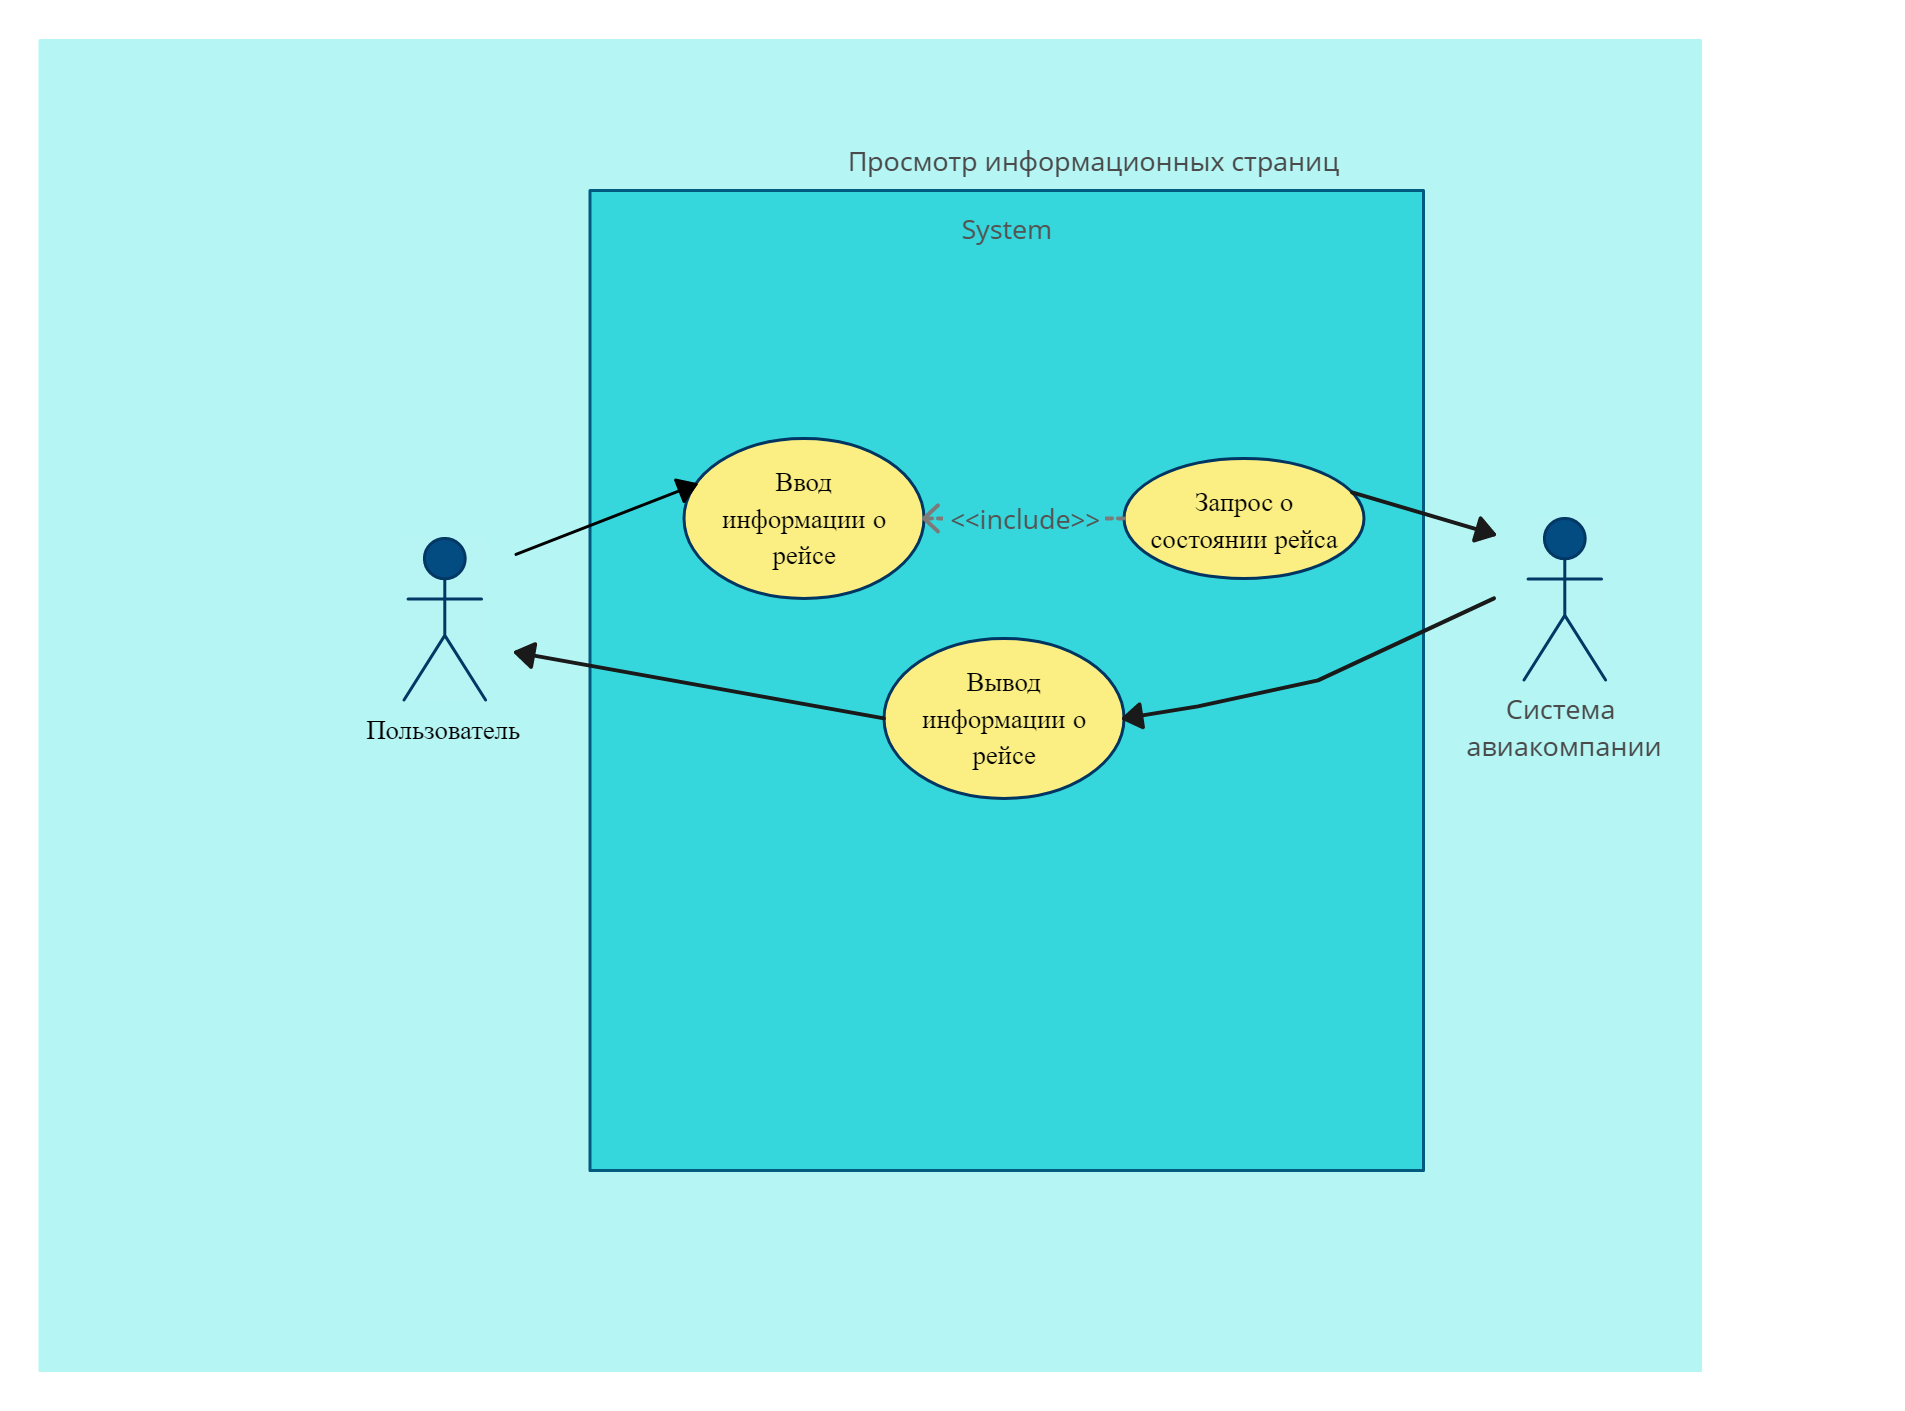
\includegraphics[width=16cm]{4-actions/Way_search.jpg}
      \centering
      \caption{Use-Case диаграмма: поиск рейса}
\end{figure}

\begin{figure}
      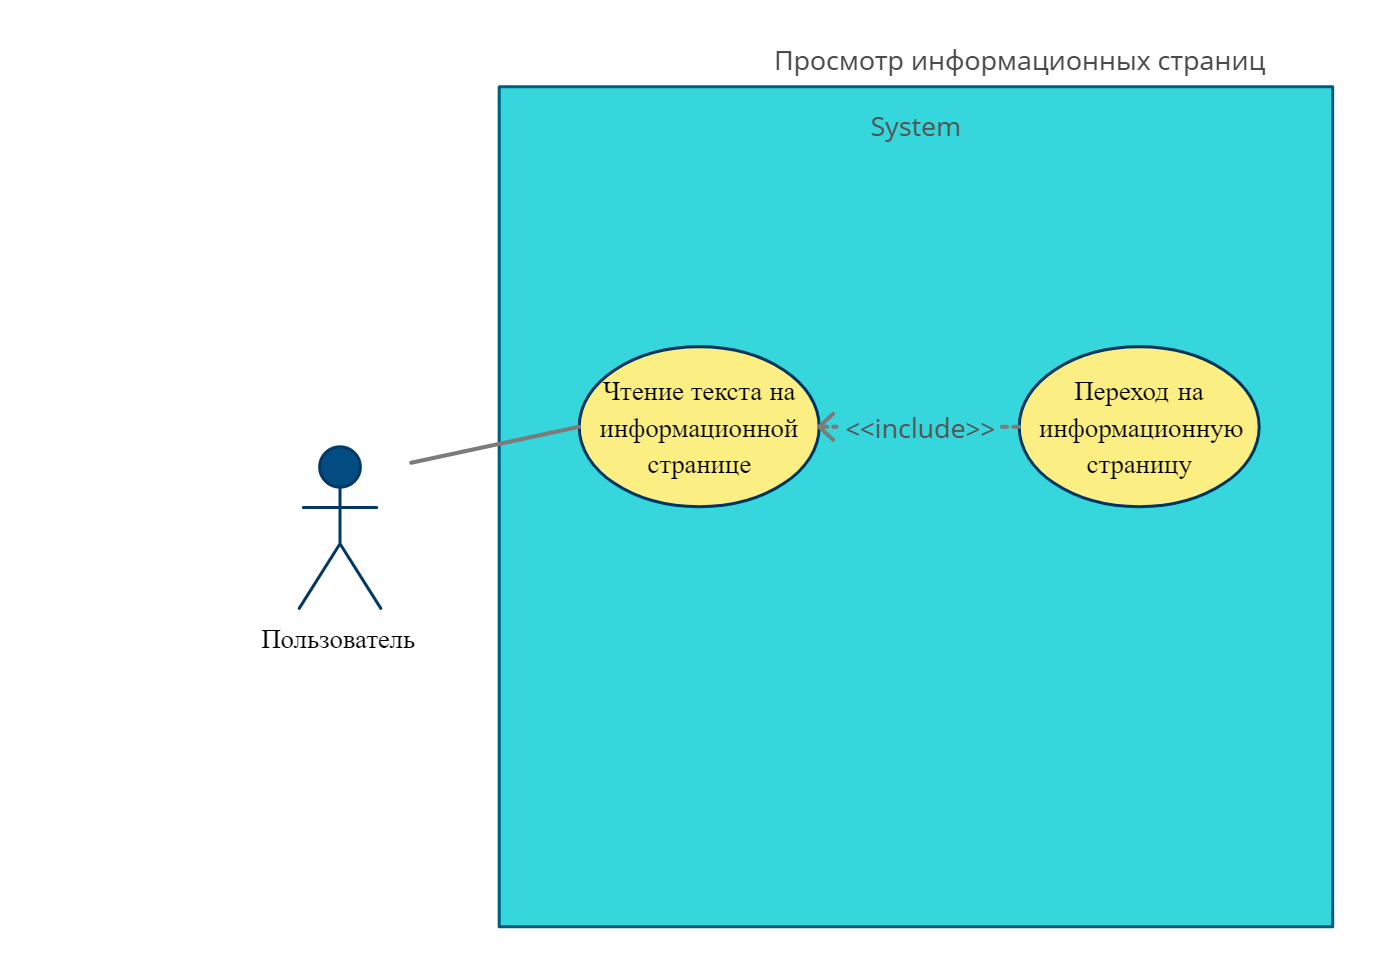
\includegraphics[width=16cm]{4-actions/Look_info_pages.jpg}
      \centering
      \caption{Use-Case диаграмма: просмотр пользователем информационных страниц}
\end{figure}

\begin{figure}
      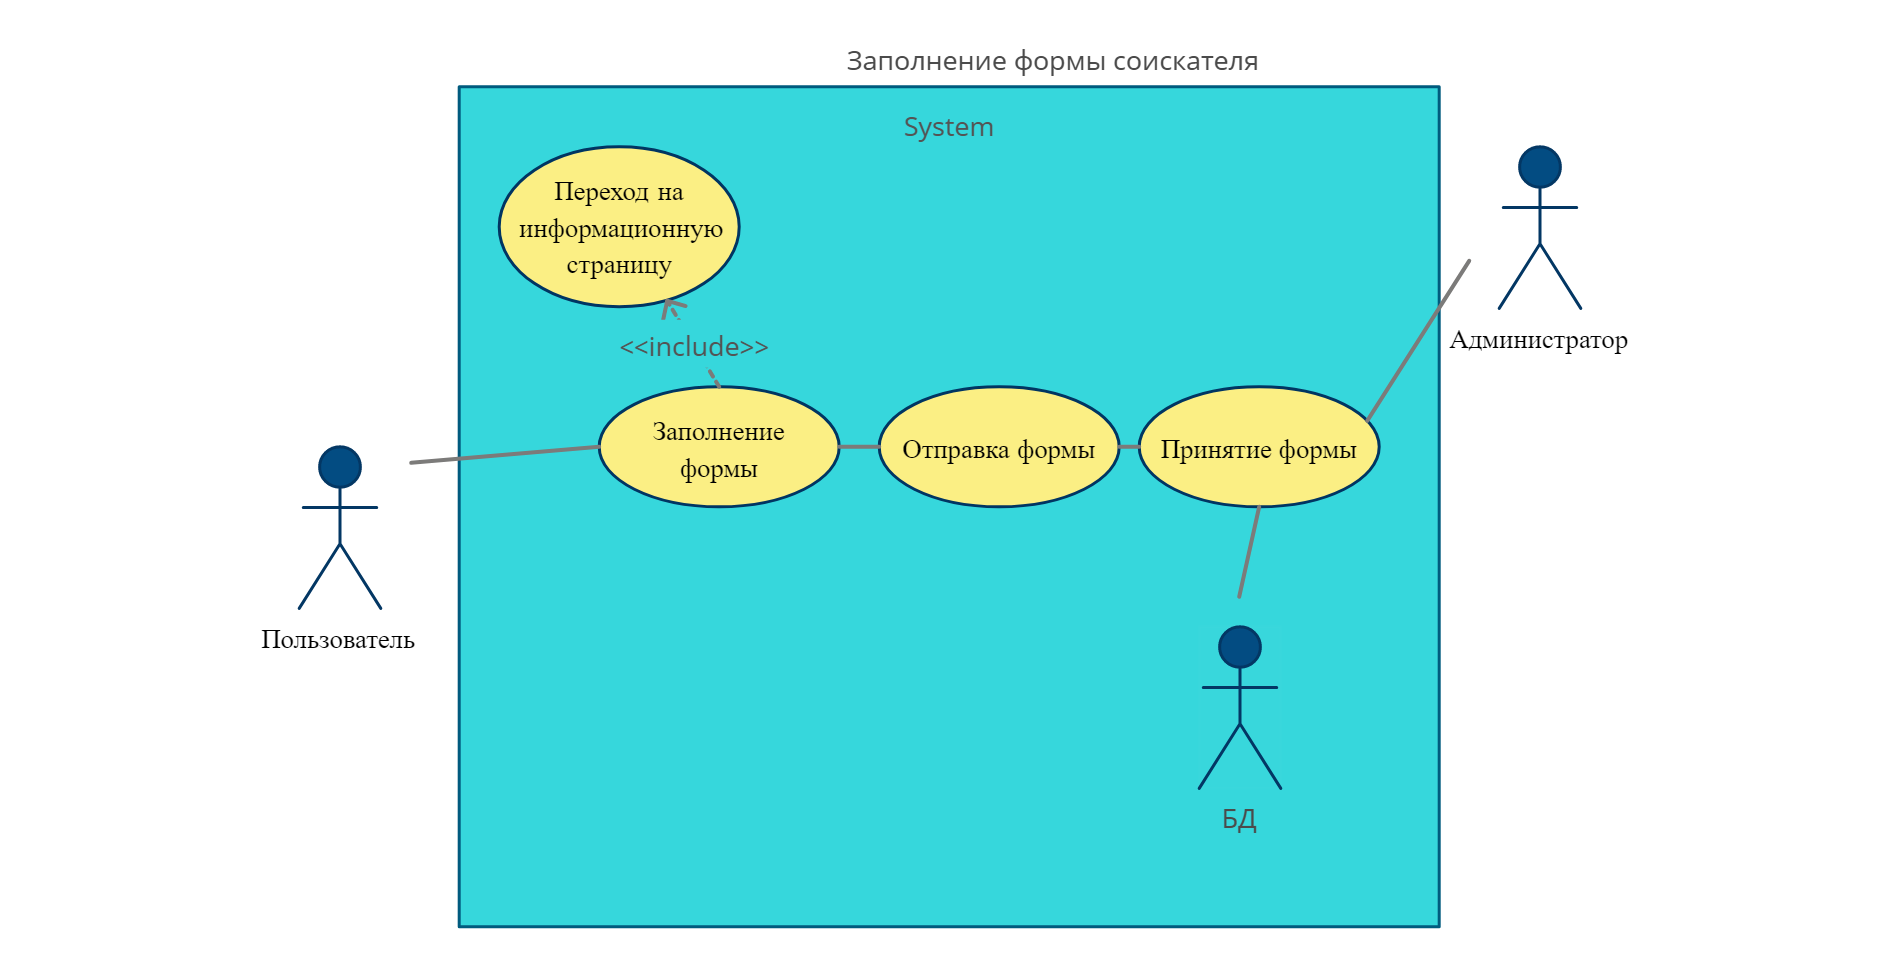
\includegraphics[width=16cm]{4-actions/Paper.jpg}
      \centering
      \caption{Use-Case диаграмма: заполнение формы}
\end{figure}

\begin{figure}
      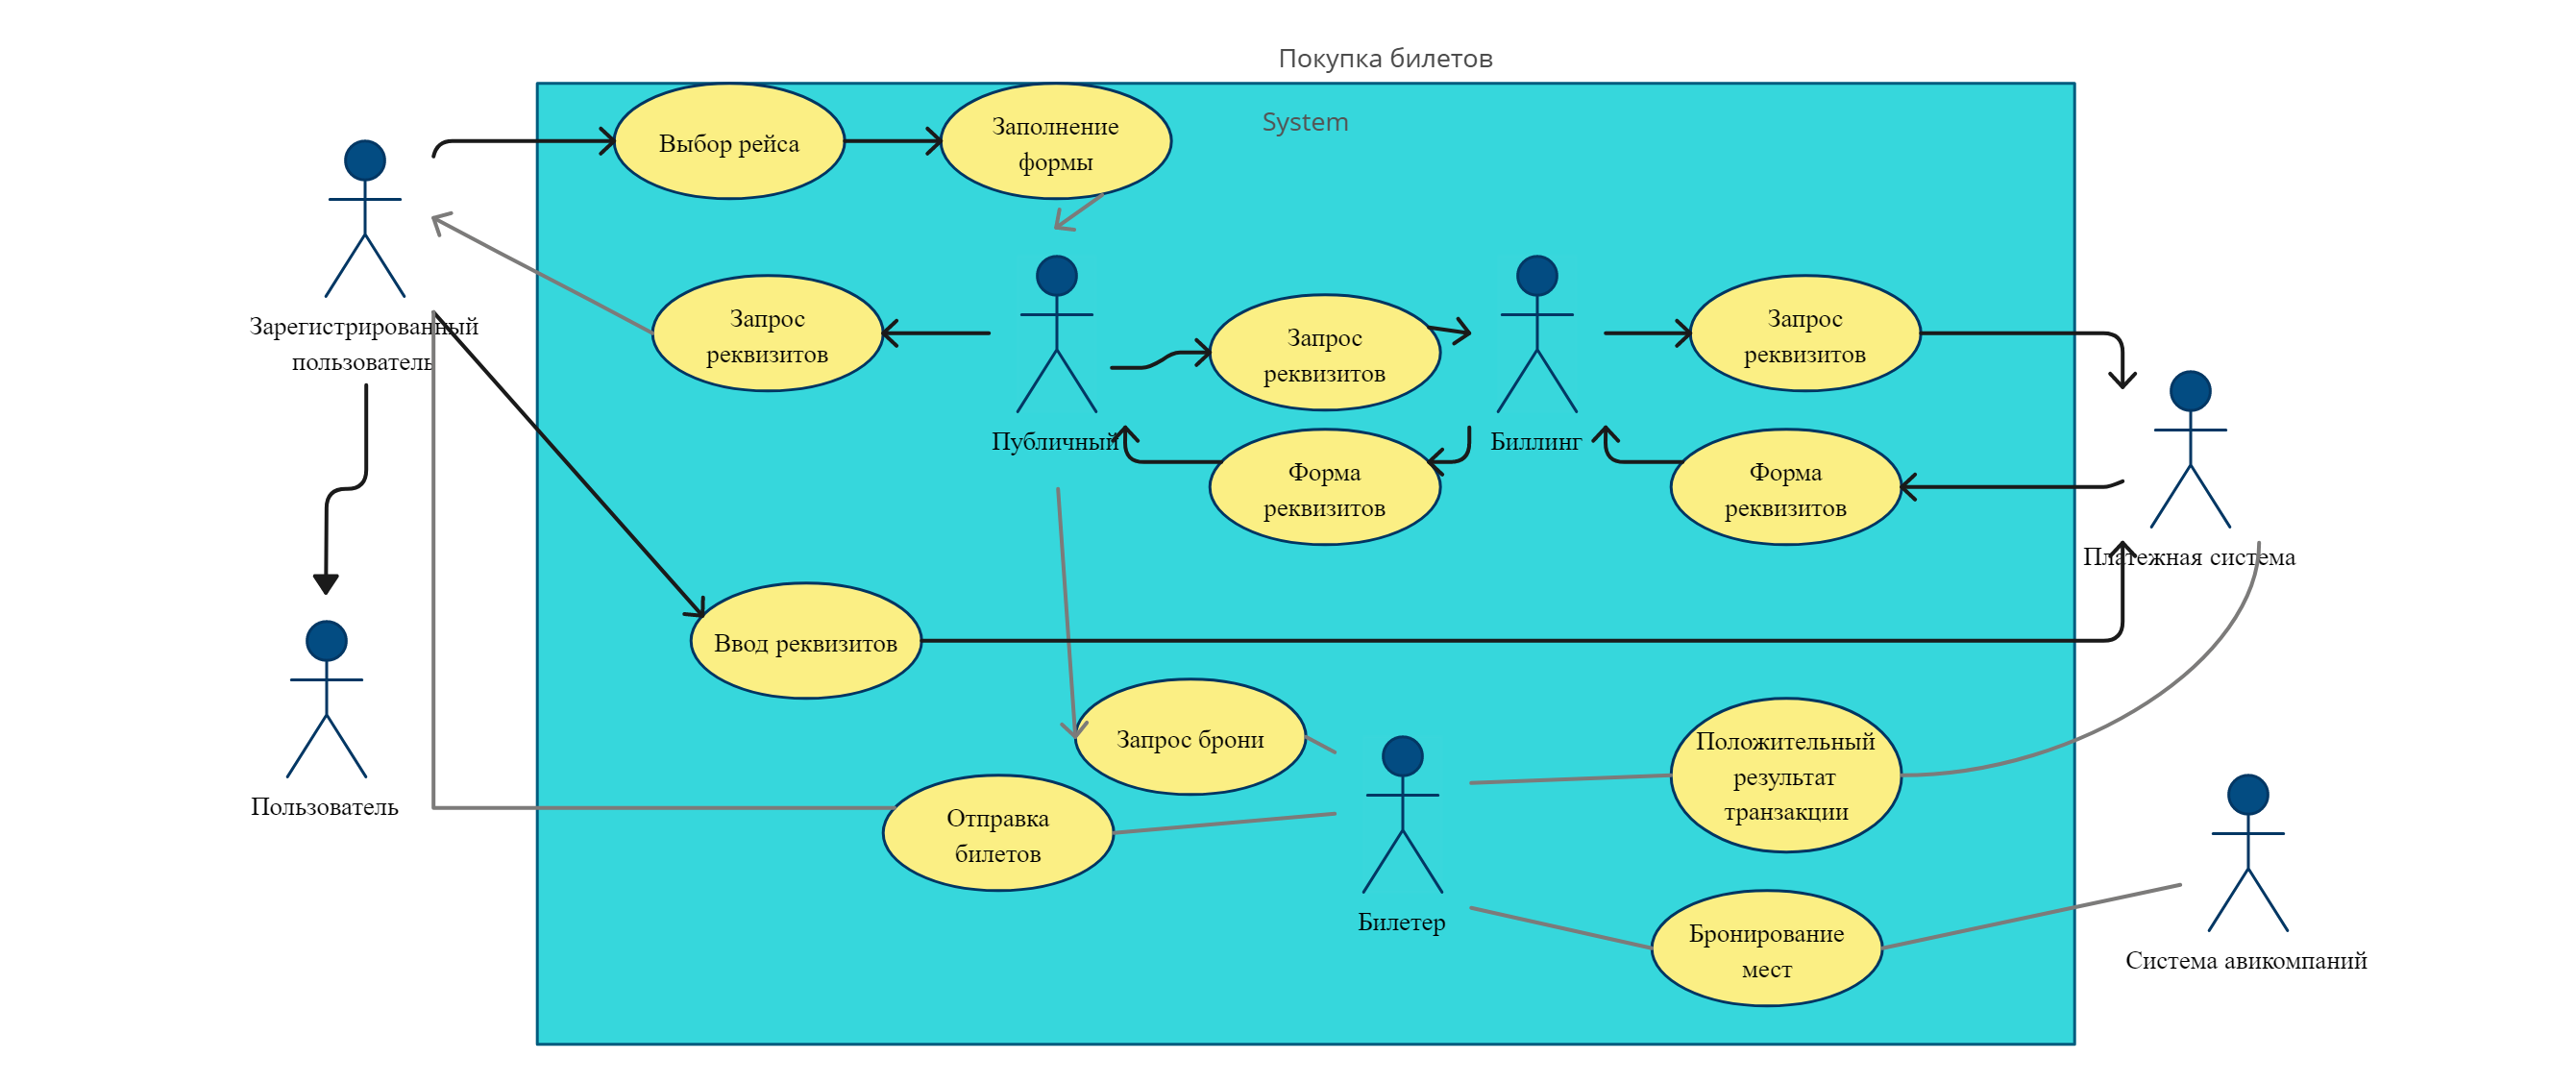
\includegraphics[width=16cm]{4-actions/Book_tickets.jpg}
      \centering
      \caption{Use-Case диаграмма: бронирование билета}
\end{figure}

\begin{figure}
      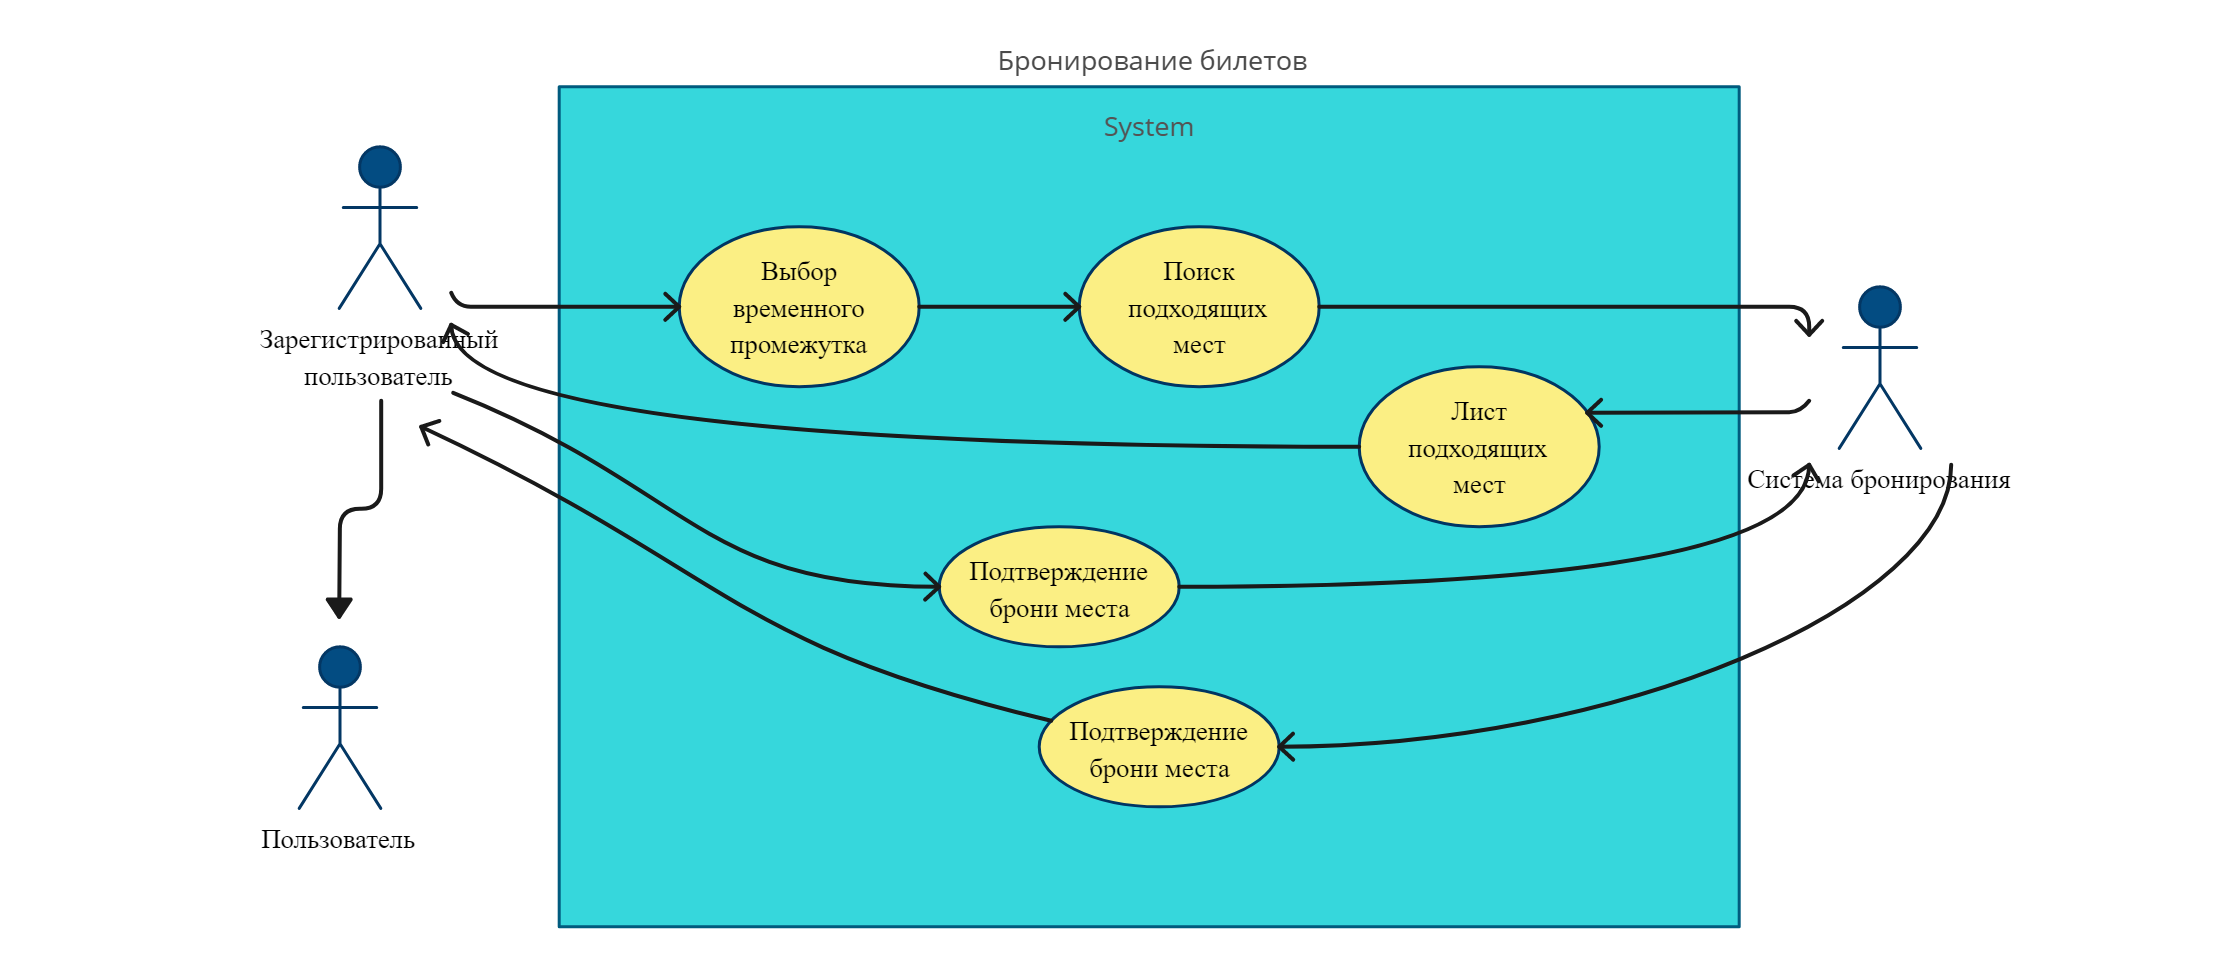
\includegraphics[width=16cm]{4-actions/Book_parking.jpg}
      \centering
      \caption{Use-Case диаграмма: бронирование паркинга}
\end{figure}

\begin{figure}
      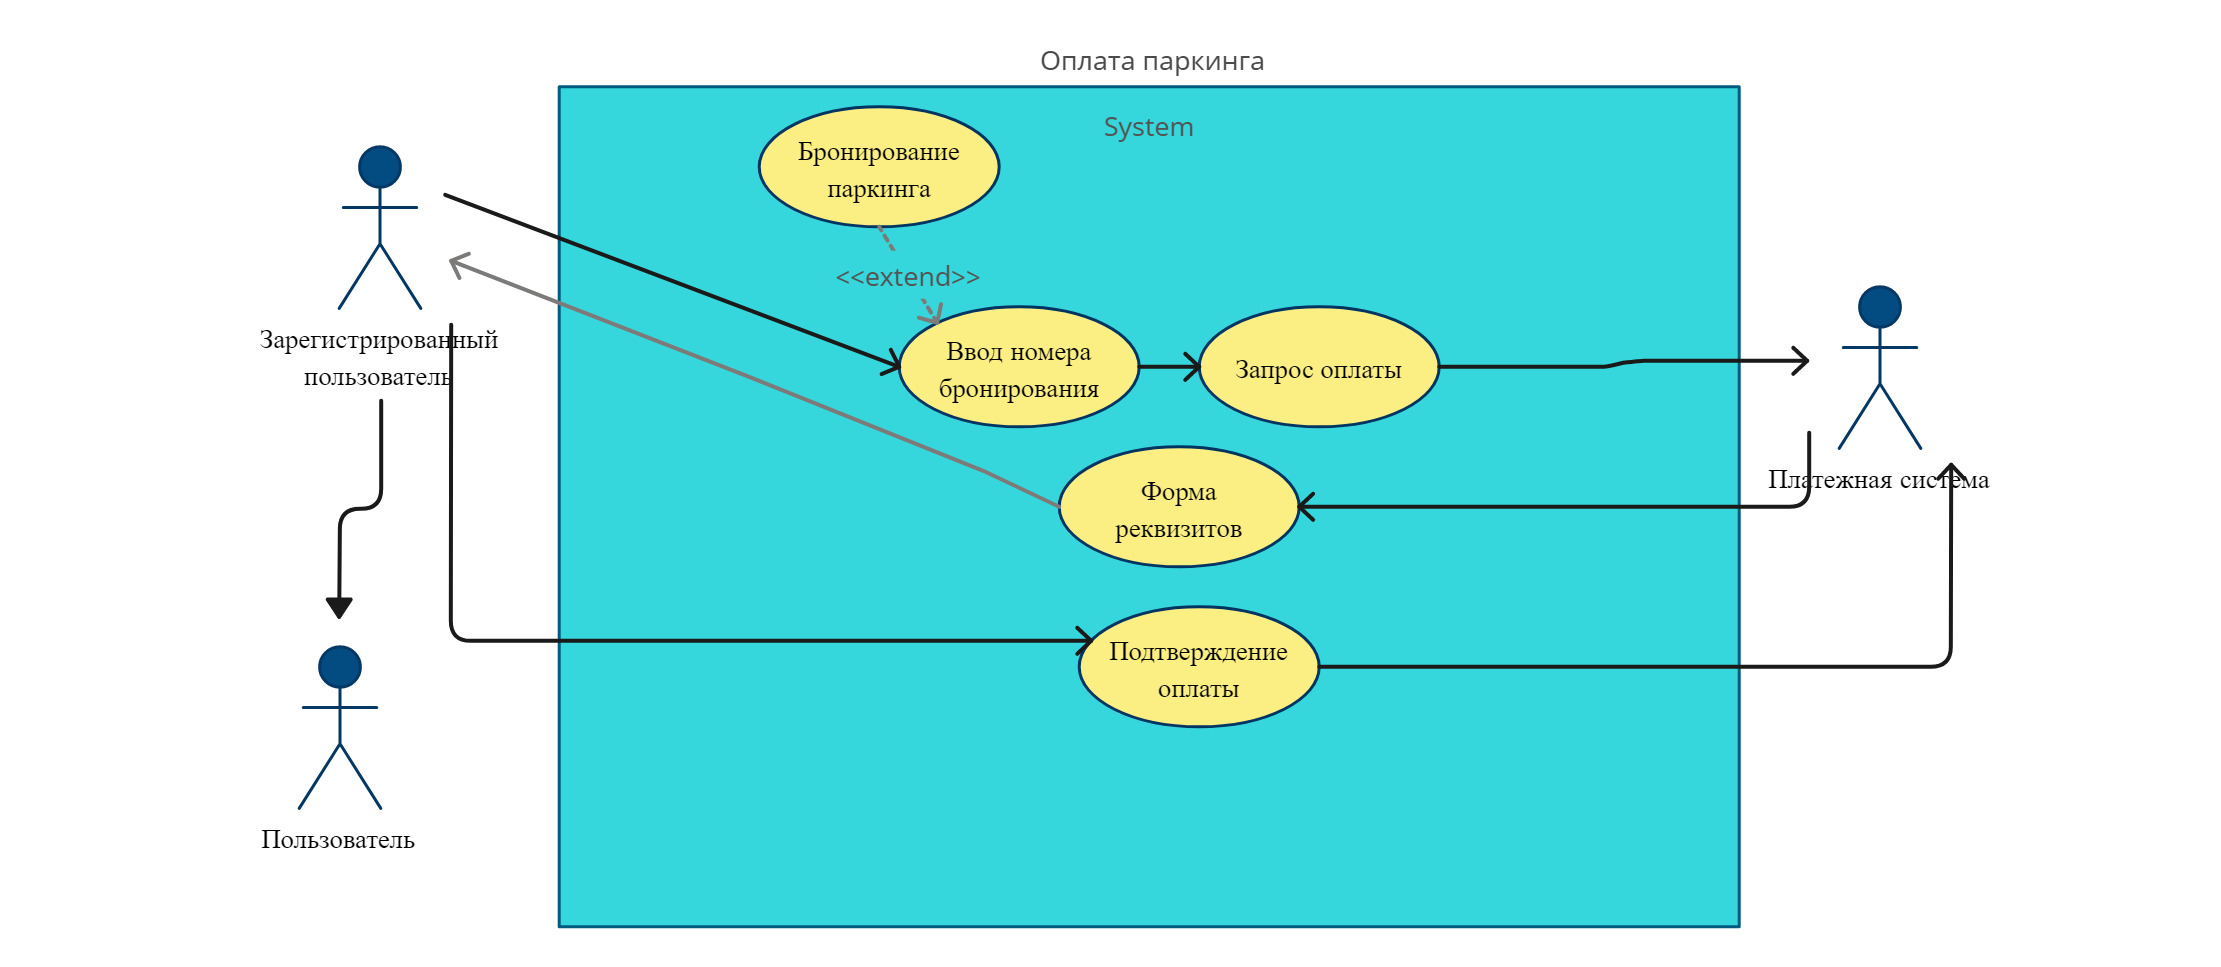
\includegraphics[width=16cm]{4-actions/Pay_parking.jpg}
      \centering
      \caption{Use-Case диаграмма: оплата паркинга}
\end{figure}

\begin{figure}
      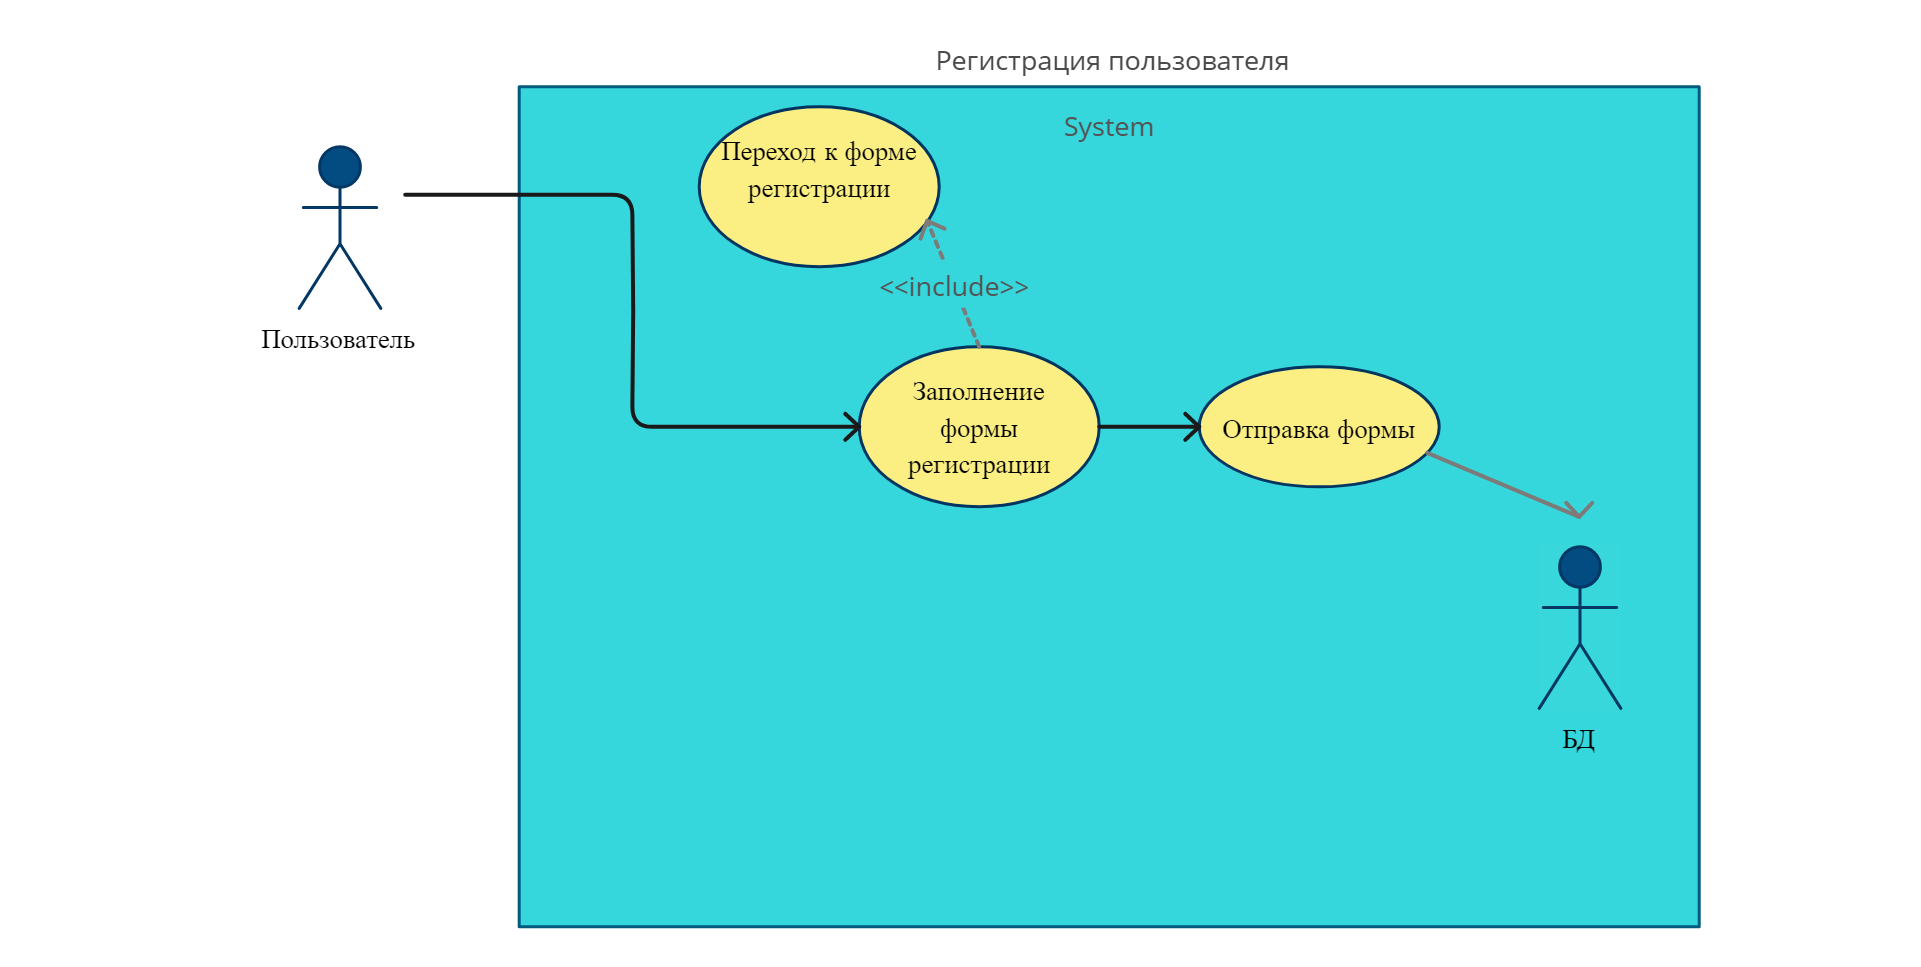
\includegraphics[width=16cm]{4-actions/Registration.jpg}
      \centering
      \caption{Use-Case диаграмма: регистрация на сайте}
\end{figure}

\begin{figure}
      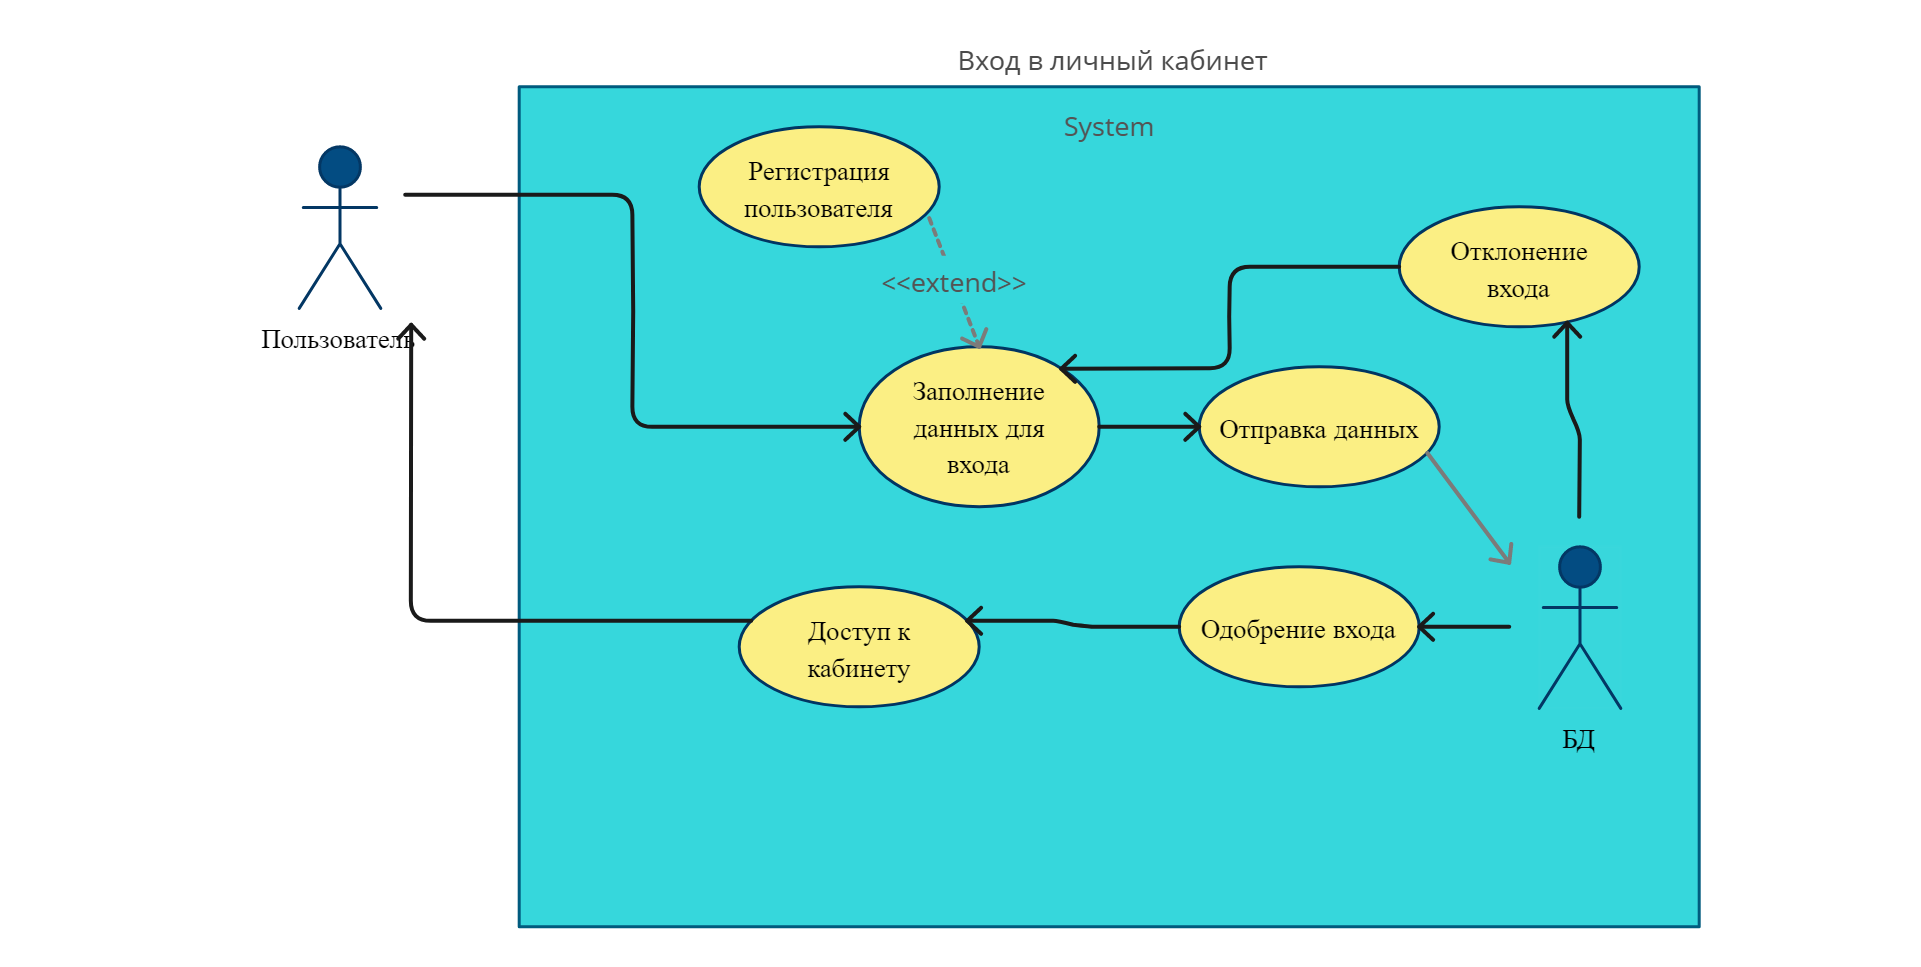
\includegraphics[width=16cm]{4-actions/Enter.jpg}
      \centering
      \caption{Use-Case диаграмма: вход в личный кабинет}
\end{figure}

\begin{figure}
      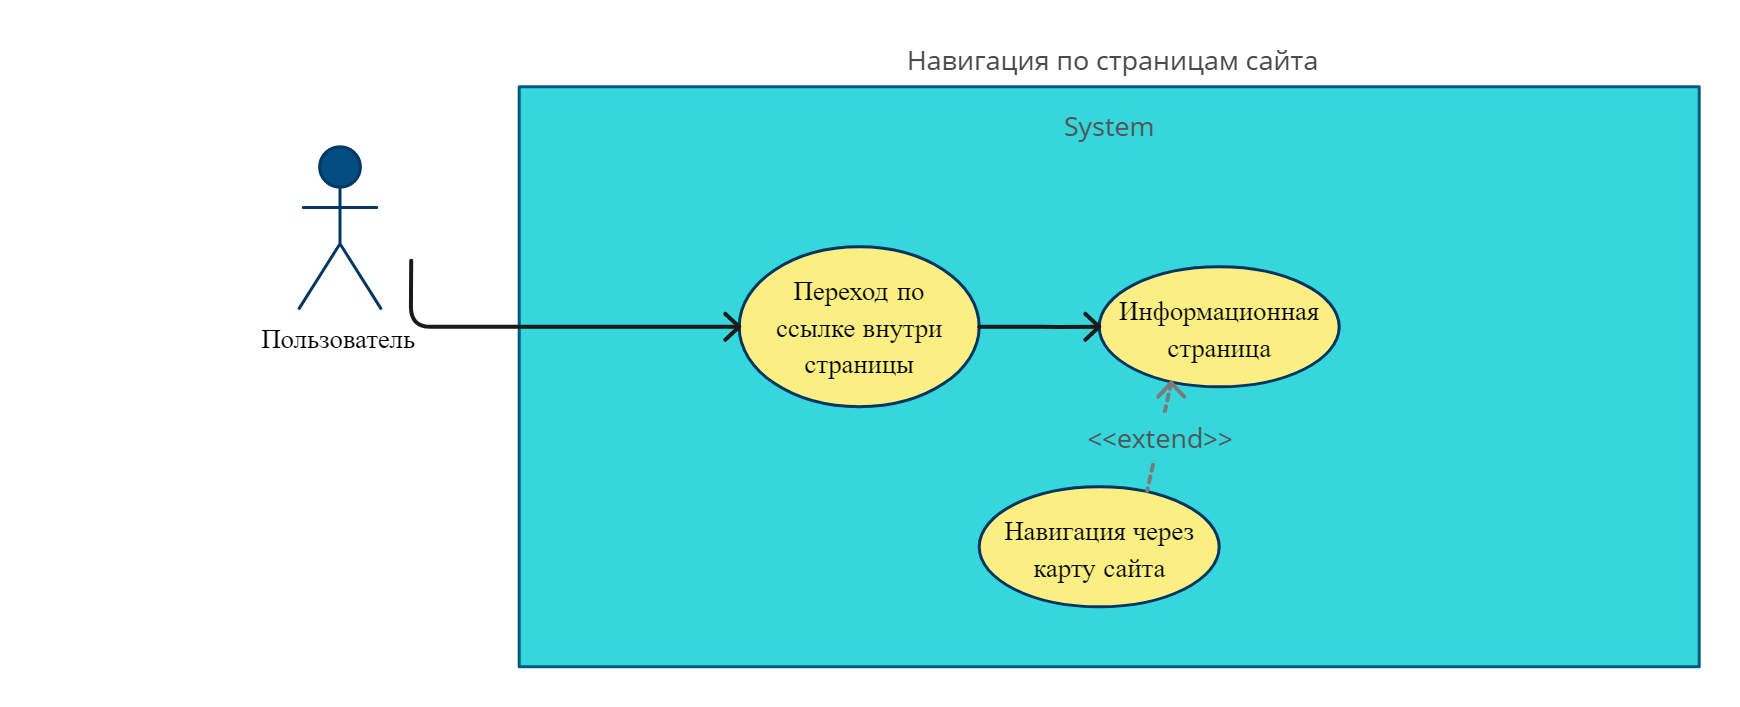
\includegraphics[width=16cm]{4-actions/Navigation.jpg}
      \centering
      \caption{Use-Case диаграмма: навигация между страницами сайта}
\end{figure}

\begin{figure}
      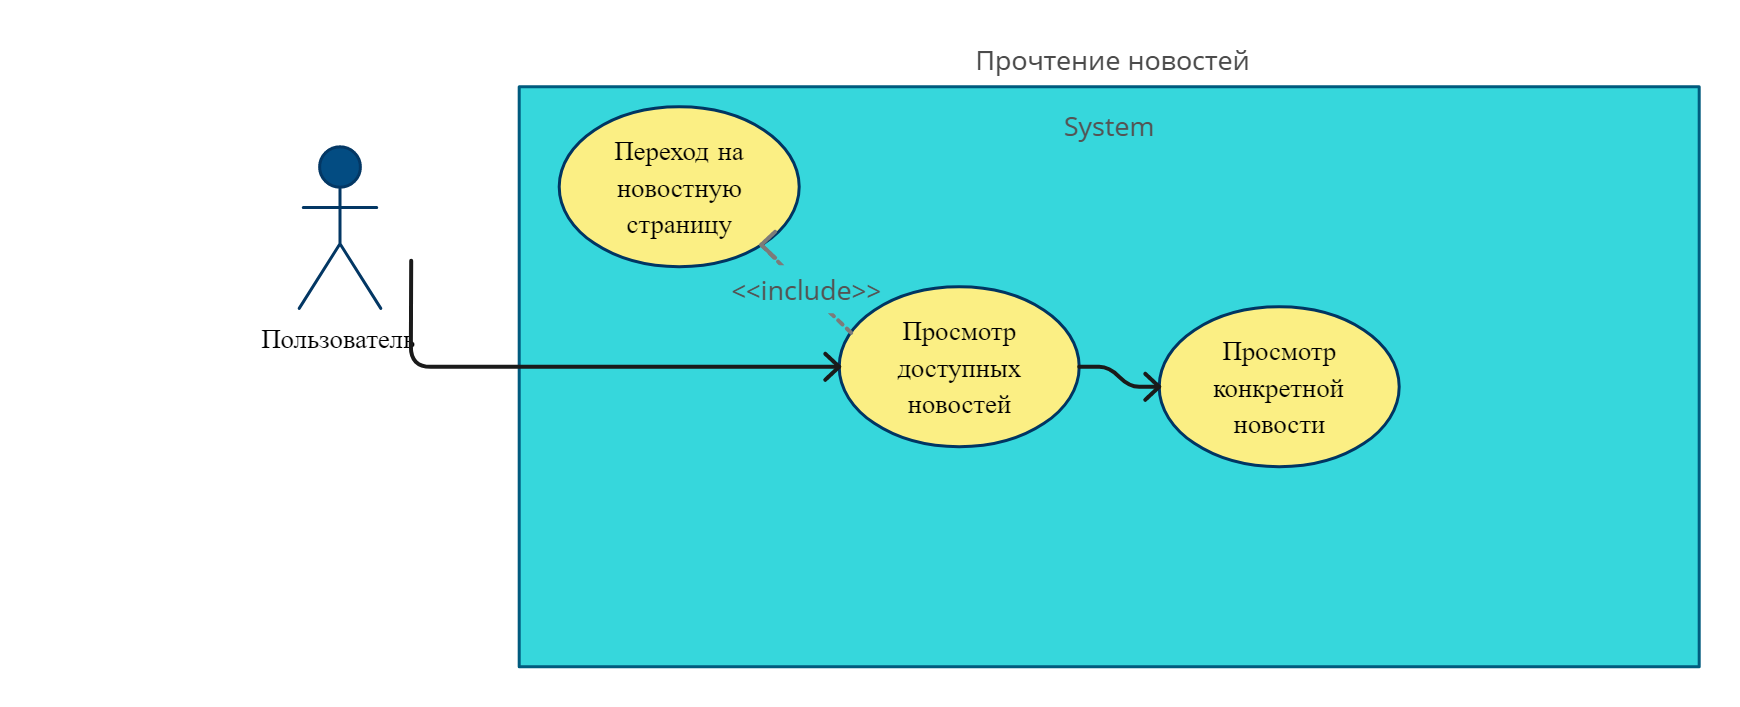
\includegraphics[width=16cm]{4-actions/News.jpg}
      \centering
      \caption{Use-Case диаграмма: просмотр новостей}
\end{figure}

\begin{figure}
      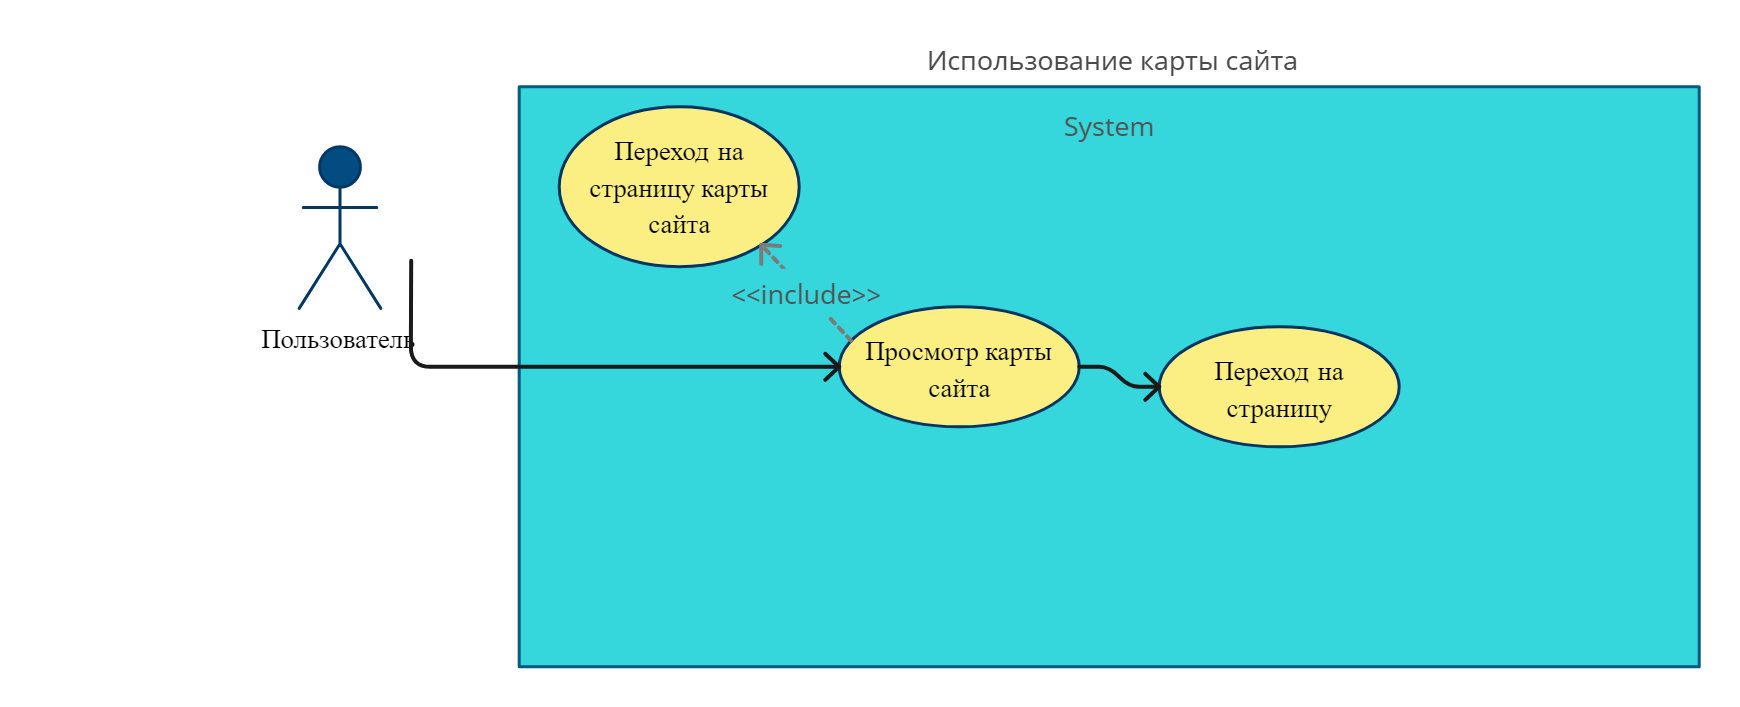
\includegraphics[width=16cm]{4-actions/App_map.jpg}
      \centering
      \caption{Use-Case диаграмма: использование карты сайта}
\end{figure}

\begin{figure}
      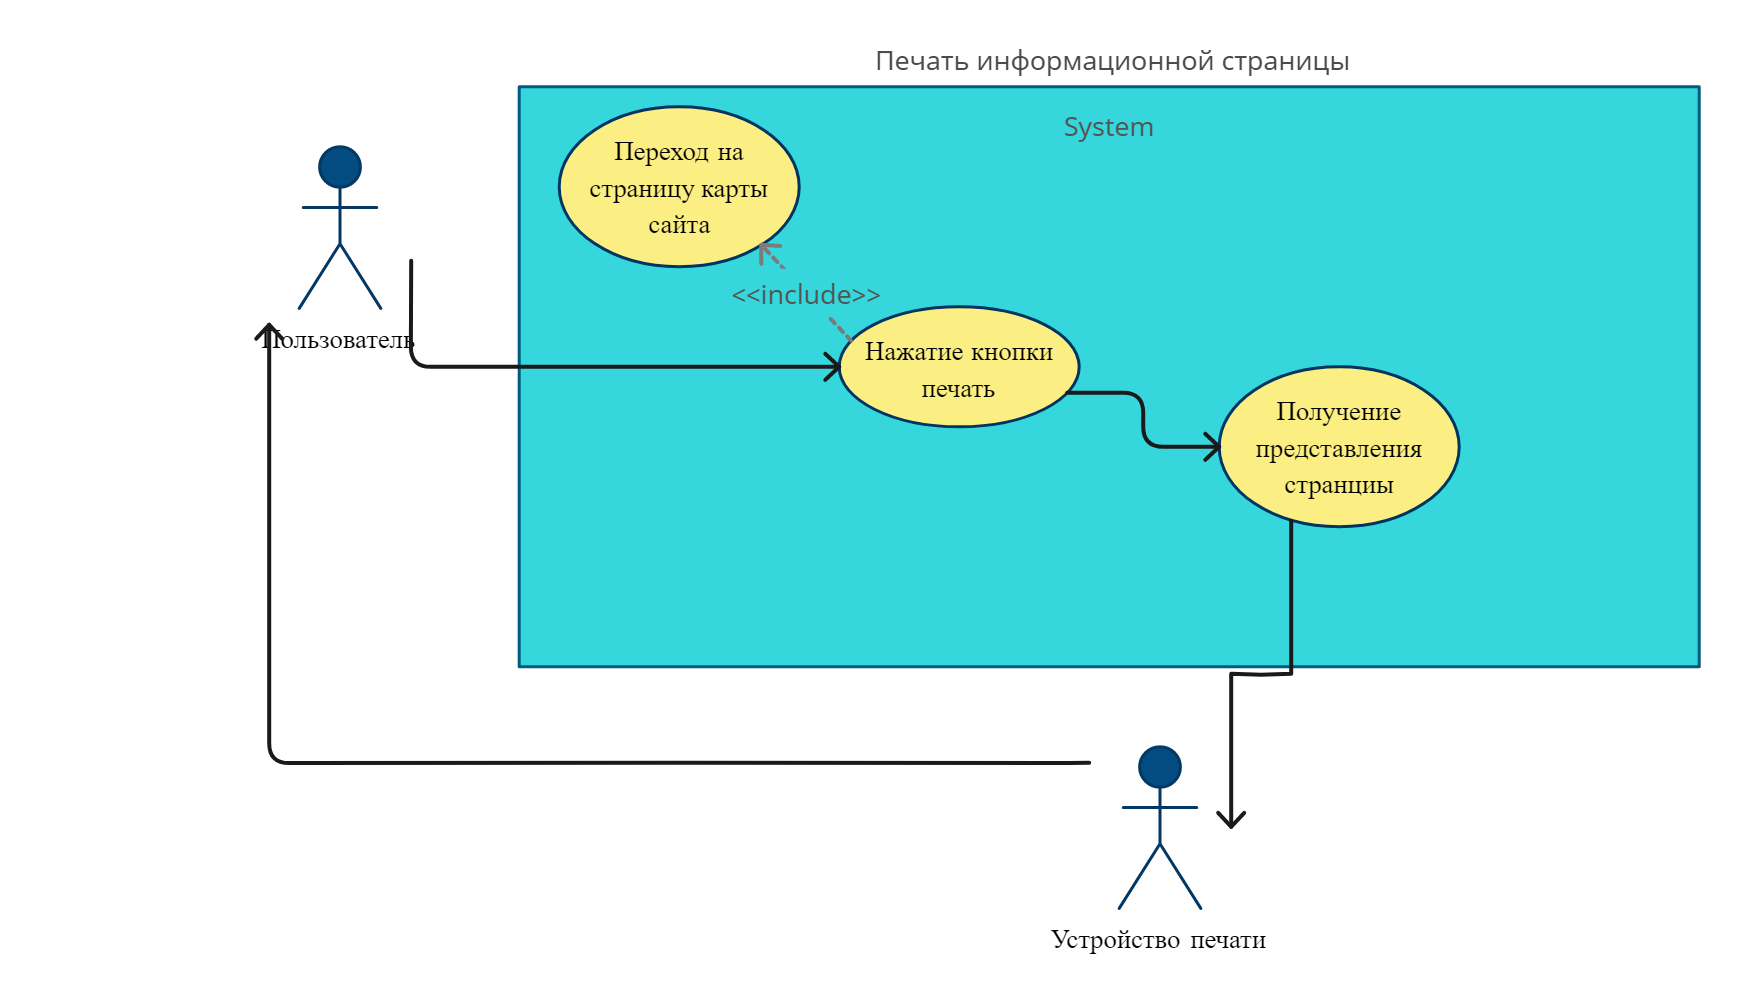
\includegraphics[width=16cm]{4-actions/Print.jpg}
      \centering
      \caption{Use-Case диаграмма: печать информационных страниц}
\end{figure}

\begin{figure}
      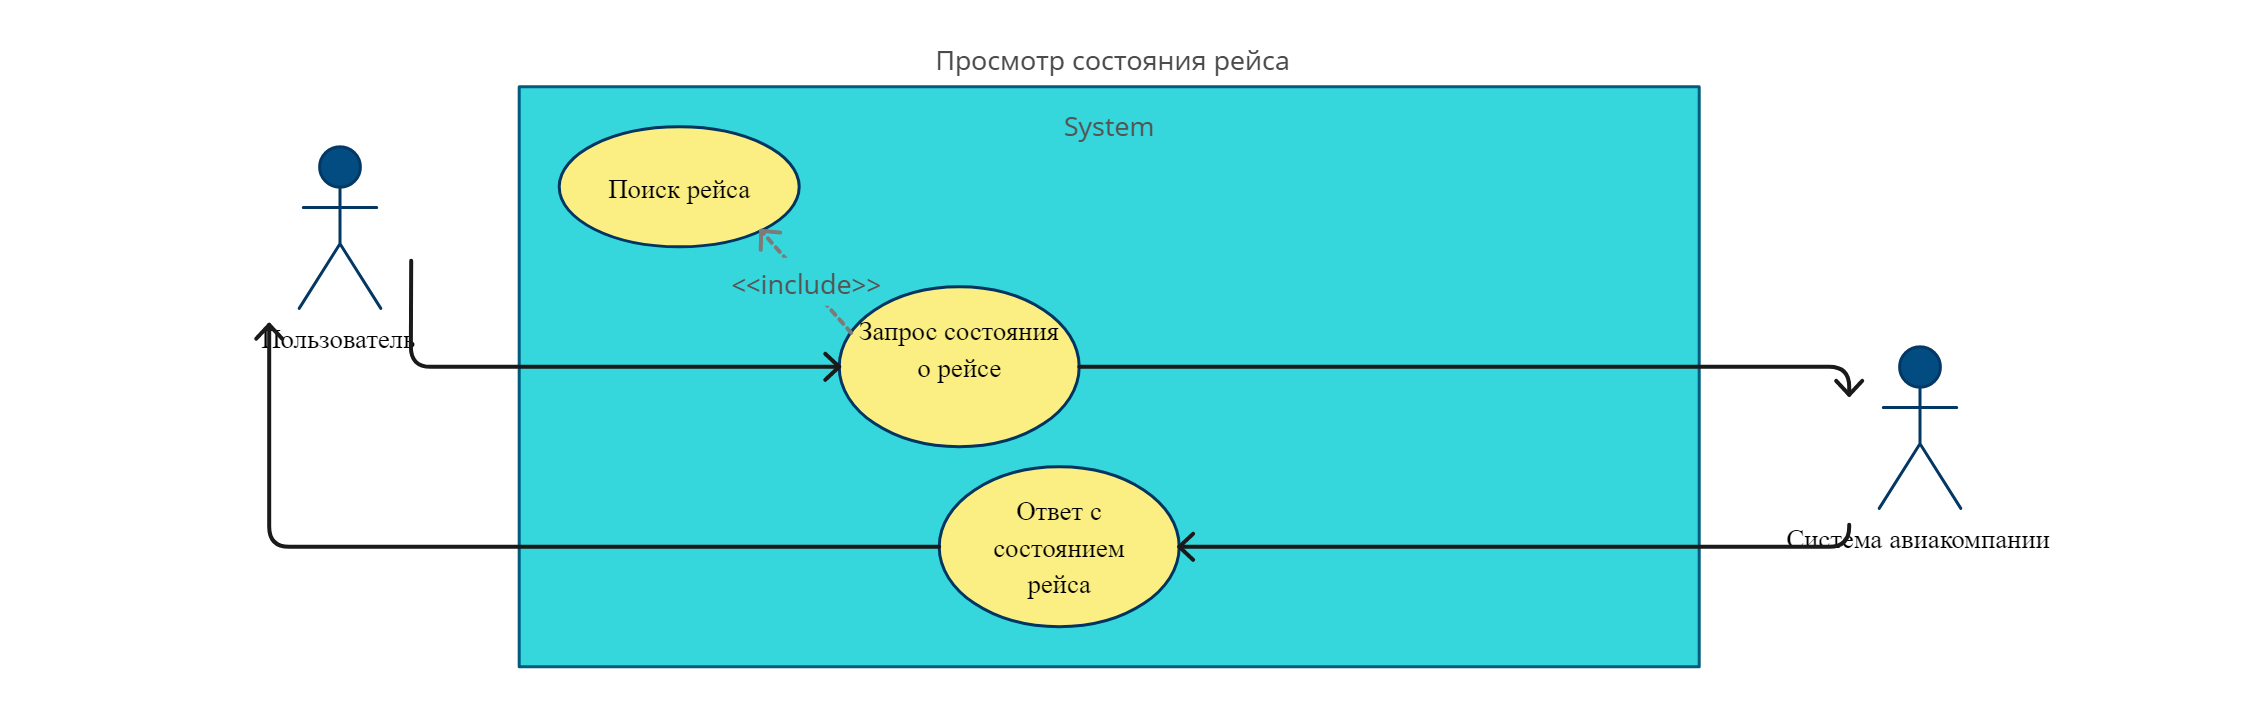
\includegraphics[width=16cm]{4-actions/Flight-state.jpg}
      \centering
      \caption{Use-Case диаграмма: просмотр состояния рейса}
\end{figure}

\begin{figure}
      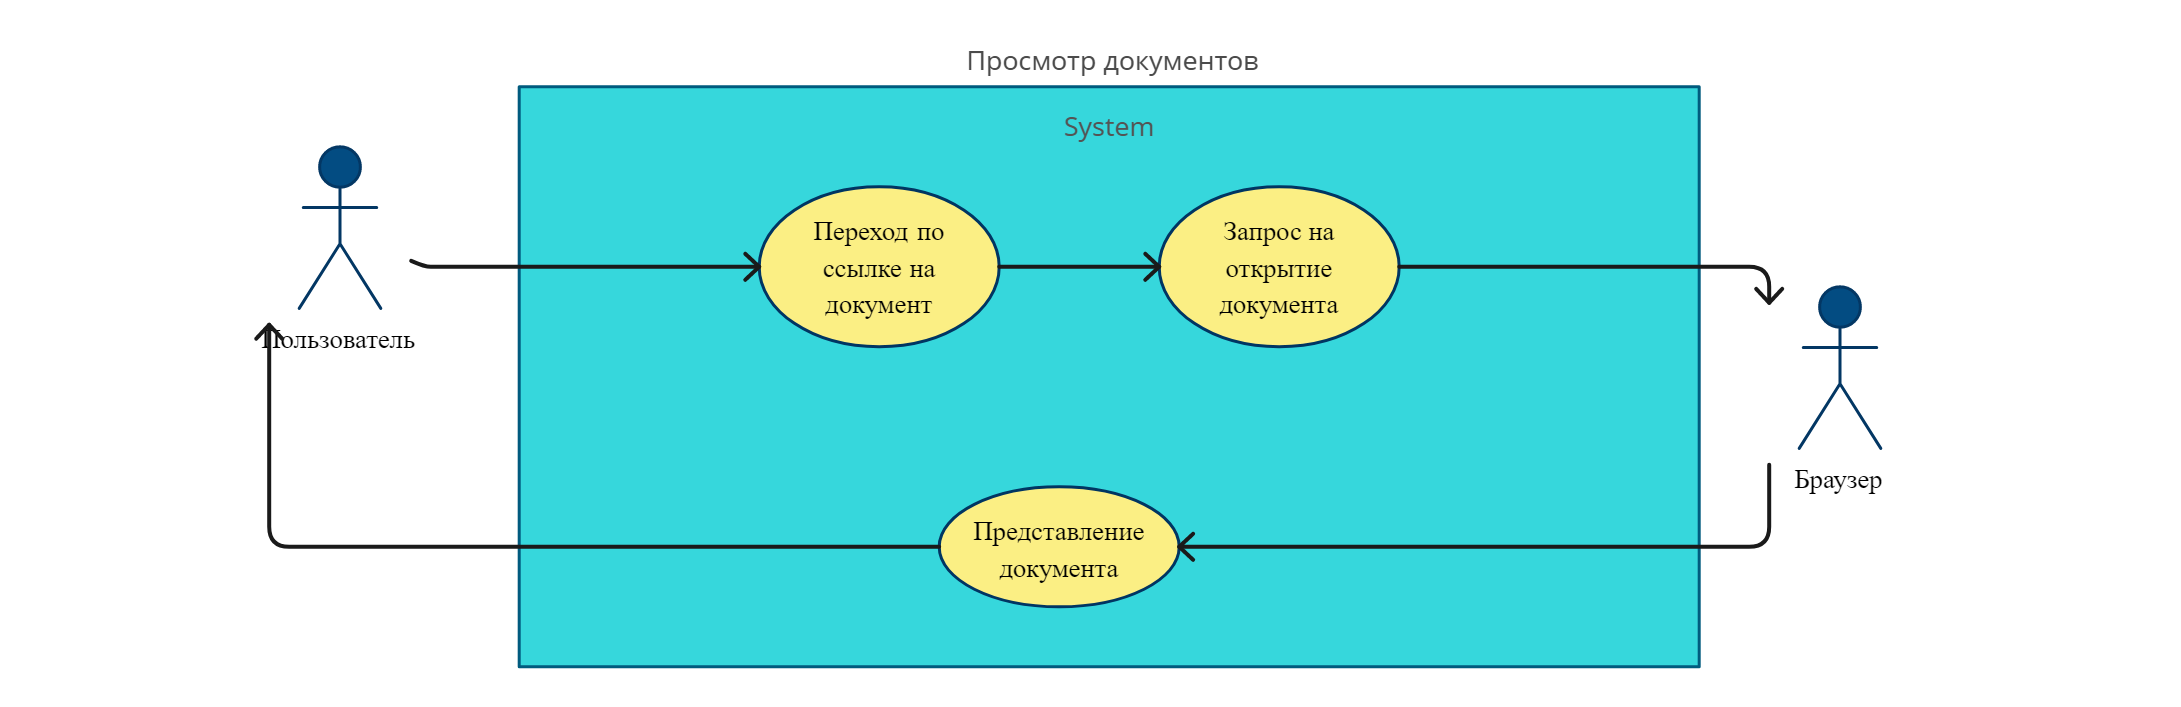
\includegraphics[width=16cm]{4-actions/Documents.jpg}
      \centering
      \caption{Use-Case диаграмма: просмотр вложенных документов}
\end{figure}

\begin{figure}
      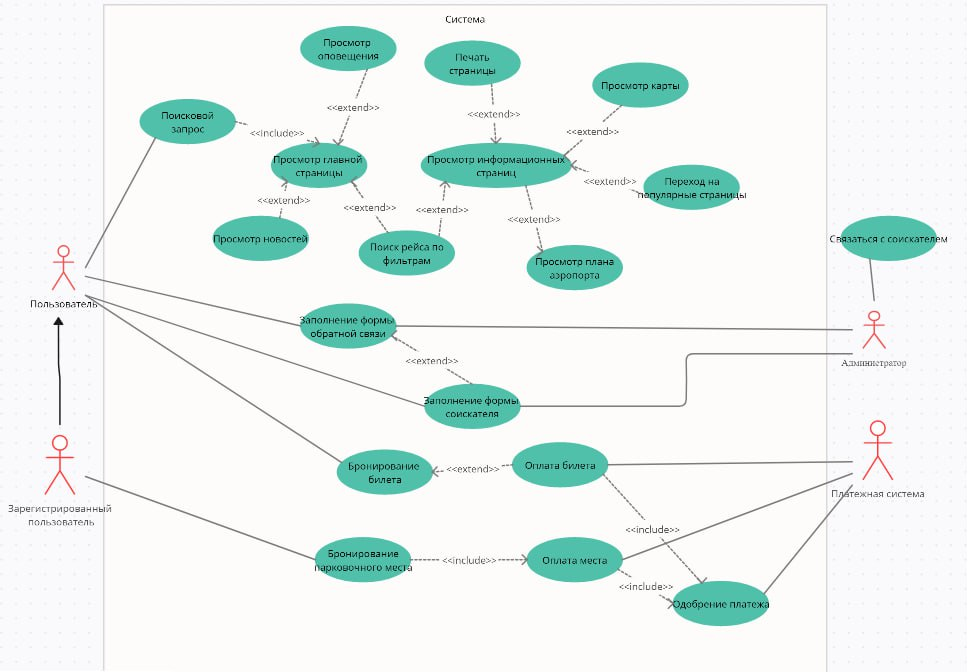
\includegraphics[width=16cm]{4-actions/use-case.jpg}
      \centering
      \caption{Use-Case диаграмма: вся система}
\end{figure}
